\documentclass[]{article}
\usepackage{tikz}
\usetikzlibrary{shadings, shadows, shapes, arrows, calc, positioning, shapes.geometric}
\usepackage{pgfplots}
\pgfplotsset{compat=1.16}
\usepackage{mathtools,amssymb}
%\input{Preamble}
%\input{(SpecialDistanceCourse}
%\input{FRAMES}
\begin{document} 
\section{Background Theory of the Firm} \label{appendix-firm-theory}

{\color{red}
% THIS COULD GO IN THE METHODOLOGY CHAPTER - we're using neoclassical firm production, more specifically.

% THIS ALSO HELPS CONNECTS THE MODEL SECTION TO THE MODEL

% MAYBE PUT WITH PART IN METHODOLOGY ABOUT NEO_CLASSICAL AND CLASSICAL ECON - THIS SEEMS LIKE SPECIFICS OF THAT BROADER PIECE
}

In this section we describe in more detail how we embed a model of diminishing returns to scale firms within an increasing returns to scale economy. We assume there are many firms operating at their optimal scale in both the rural and urban sector, but the production function of the urban firm is augmented by the term $N^\gamma$. 

% NOTE ON EXPONENTS

We distinguish the parameters of production functions for rural and urban firms and for the city as a whole. We assume that rural and urban firms use the same Cobb-Douglas technology ${y_R}=A_Fk^{\alpha_F}n^{\beta_F}$. The difference is that the urban firm enjoys a multiplicative agglomeration externality $N^\gamma$, so ${y_U}=A_FN^\gamma  k^{\alpha_F}n^{\beta_F}$. We assume $\gamma$ is zero for the rural firm. 

We set $\alpha_F$ and $\beta_F$ as a parameters for firms. We assume that $\alpha_F+\beta_F<1$, so that firms exhibit decreasing returns to scale.  We then calculate a value for $\gamma$ consistent with the strength of the observed agglomeration effects. 

With these assumptions we have an aggregate production function for the city that exhibits increasing returns to aggregate labour, $N$,  which we write $Y=AN^\beta$. Where $\beta$ for the city as a whole, differs from $\beta_F$ for the individual firm, because of agglomeration effects. 

In the model, firms adjust labour and capital to the profit-maximizing levels given the wage. % and size of the aggregate workforce. We now describe the behaviour of the firm sector. 
%In each period we have the size of the existing workforce $N$ and the number of firms $F$ and $k_t$.  %\footnote{We also inherit the size of the existing firms. We can simplify by assuming firms do not change their capital stocks as wages change. This would be incorrect but would do as a first approximation. }
Firm output is given by:

\begin{equation}
    {y}_t= A_FN_t^\gamma k_t^{\alpha_F}n_t^{\beta_F}, \label{eqn-urban-firm-output}
%    Y_t=& N_ty^\gamma y^\]  
\end{equation}
where $\gamma$ is drawn from the agglomeration literature.% but $A$ must be calculated to.

The output equation, differentiated with respect to  $n$, yields the marginal product of labour (MPL). Simplifying by substituting back in $y_t/n_t$. %n^epxonent -1 pull out and put n underneath
\begin{equation}MPL_{t} = \frac{\beta_{F}P{y}_{t}} {n_t}. \label{eqn-urban-firm-mpl}
\end{equation} 
Following the rule for profit-maximizing firms, the firm should hire until the marginal product of labour is equal to the wage, $MPL_t= {\omega_t + \psi +}$ overhead. This describes the individual firm's demand for labour, which doesn't take into account the overall effect on productivity due to every other firm increasing their labour force at the same time. 

Firm demand for labour determines the wage, which then drives labour supply. Firms are identical, so the number of firms increases to absorb the labour supply.

%\begin{equation}N_{exist,t+1}^{target} = \frac{n^{target}_{t+1}}{n_{t}} N_t\end{equation}   


Firms also adjust their capital stock as the relative price of labour rises. We can compute the marginal product of capital in the same way we calculated the marginal product of labour, by differentiating the output equation with respect to capital:
\begin{equation} MPK_t = \frac{\alpha_{F}\ P{y}_{t}}{k_{t}}. \label{eqn-urban-firm-mpk}
\end{equation} 
The revised $MPK$ should equal their cost of capital, $r_F$. % and adjust the capital stock so that the MPK$_t$ is equal to $r_F$. 

\begin{equation}k_{t+1}^{target}= \frac{\alpha_{F}\ P{y}^{target}_{t}}{r_F},\end{equation}
where  $y_t^{target}$  is calculated using $n^{target}_{t+1}$. % into Equation~\ref{eqn-urban-firm-output}.

% It is based on planned output using planned labour rather than the labour available in the period, so we begin with the marginal productivity of labour equation, 
% which gives us 


% \begin{equation} n^{target}_{t+1}= \frac{\beta_F {y}_{t}}{\omega_t + \psi} \label{eqn-urban-firm-target}
% \end{equation}

%\subsubsection{number of firms}  Firm formation uses current variables to set number of firms for the next period. Decisions to enter or leave in the next period are based on current values. 
% \begin{equation}F_{t}=\frac{N_{t-1}}{n^{target}_{t-1}}\end{equation}
% . An increase in the number of firms adds to labour demand: 
% \begin{equation}
%     new\ firm\ demand = n^{target}_{t-1}(F_{t}-F_{t-1})
% \end{equation}


% \subsubsection{Including  urban labour demand for new firms}
% If firms are making a profit, standard micro theory tells us new firms will enter the market. % $dF/dt >0$. % The converse is true as well: $MPK_t > r_F \rightarrow dF/dt <0$. 
% Theory tells us nothing about how many firms will enter, %but suggests that this adjustment will be slower than the adjustment of the labour market target adjustment rate, $\frac{n^{target}_{t+1}}{n_{t}}$. 
% so we (arbitrarily) assume the ex-ante growth in the desired number of firms is the same as the  target growth rate of the firm's  force.\footnote{We could use a more complex function that responded to a proxy for profits, such as $Z=\frac{MPL-(\omega+\psi)}{\omega+\psi}$.} 

% % \begin{equation}
% % F_{exist,t+1}= 0.25\frac{n^{target}_{t+1}}{n_{t}}F_t
% % \end{equation} 

%  \begin{equation}
% F_t^{target}= \frac{n^{target}_{t+1}}{n_{t}}F_t
% \end{equation} 

Taking into account firm growth and growth in the number of firms the target towards which the population would be adjusting  is: 

 \begin{align}
N_t^{target}&=F_t^{target}n_t^{target}. 
% \\
%  %           &= \frac{n^{target}_{t+1}}{n_{t}}F_t\  n_{t+1}^{target}\\
%             &= \frac{(n^{target}_{t+1})^2}{n_{t}}F_t
\end{align} 
% where $n^{target}_{t+1}$ is given by Equation ~\ref{eqn-urban-firm-target}.  
The precise value of the hypothetical target is less important because the adjustment is spread over several periods. % We assume a partial adjustment of the form:




% \subsubsection{Total aggregate urban labour demand of existing and new firms $N_{T,t+1}^{target}$} 
% Total labour demand will be

%However, in the agent model, the agents decide whether to work in the urban market individually, considering the wage and transportation costs.


% \begin{equation}
% N_{total,t+1}^{target} = F_{t+1}n^{target}_{t+1}\end{equation}  

% Target employment 
% This is used in below to calculate next period employment and wage premium.




%\footnote{There are additional second-order adjustments we could consider. Firms will increase their capital stock and reduce their labour force in response to rising labour costs. At the same time, increasing employment will shift the marginal productivity curve outward.}


% \subsubsection{Number of firm adjustment} 
% \begin{equation}
% F_{total, t+1}=\frac{N_{total,t+1}^{target}}{n^{target}_{t+1}}
% \end{equation}
% This adjusts over time, keeping the firm labour force near the optimal level. 










 % (This should be the same result as  multiplying $n^{target}_{t+1} \times F_{t} $.)

% Y is produced with the year's realized workforce.

\section{The adjustment process}
%In conventional economic analysis of markets with many firms, in order to compute an equilibrium, firms are treated as price takers. 
In an ABM equilibrium is not imposed. Realistically, firms must raise their wage offer to get more workers. New workers have to be induced to enter the market. %We do not model the wage bargaining process, however. We simply introduce a plausible adjustment process that takes account of both the firm's demand and the actual supply constraints.  

%Given target labour demand, firm numbers, firms must adjust the wage to bid for new workers.

%The simplest version of our story is that the profit-maximizing price-taking firms make a decision to expand employment at a given wage. They do so because realized labour productivity is higher than expected,  a result of agglomeration effects.

%To capture the iterative dynamics of the market, 
% Individual firms have limited market power and we model of them as thinking of themselves as price-takers. 
%Firms need not take into account that if they all increase labour demanded, wages must rise. 
We know that the actual supply of labour in this model is constrained by the transportation cost. In our ABM with uniform density, the population is simply the square of twice the distance that workers will travel for a given wage premium: $N=density*2(\omega/c)^2$.\footnote{The greatest distance  an agent will travel to work in the city is $\omega/c$. This results in an area of $2(\omega/c)^2$. With the block metric for travel, the area is a square with a diagonal length of $2\omega/c$. Using Pythagoras the side of the square is $\sqrt(2)\omega/c$, and the given area is the square of that value.} %Aggregate target employment is then $N_{t+}^{target} = F_t^{target} n_t^{target}= density*2(\omega/c)^2$. 
Solving for $\omega$ in terms of $N$, %=F_{t+1}^{target} n_{t+1}^{target}$ 
gives us the target urban labour supply curve, 

\begin{equation}
   \omega= c\, \sqrt{\frac{N}{2 * density}}
\label{eqn:Labour-supply}\end{equation}

For a given $N^{target}$ we can calculate the required wage premium
\begin{equation}
   \omega^{required}= c\, \sqrt{\frac{N^{target}}{2 * density}}
\label{eqn:Labour-supply2}\end{equation}


\begin{figure}
    \centering
   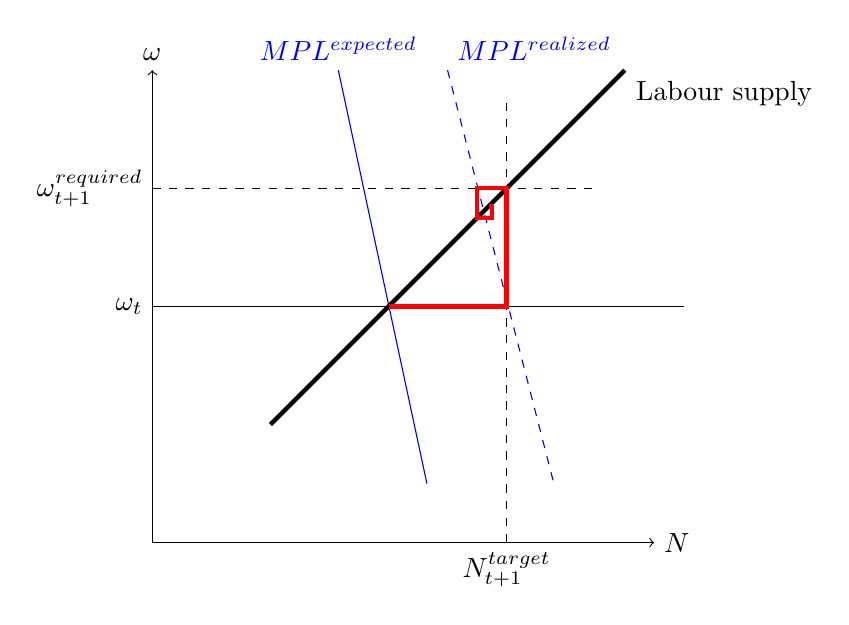
\begin{tikzpicture}[scale=.75]
% \draw[style=help lines,step=0.5cm] (-4,-4) grid (4,4)        [step=0.5cm]; %   (1,2) grid +(1,1);
% \node at (0,0){x};
 \draw[->] (-4,-4) -- (4.5,-4) node[right] {$N$};%
 \draw[] (-4,0)node[left] {$\omega_t$} -- (5,0);
\draw[dashed] (-4,2)node[left] {$\omega_{t+1}^{required}$} -- (3.5,2);
\draw[dashed] (2,-4)node[below] {$N_{t+1}^{target}$} -- (2,3.5);

 \draw[->] (-4,-4) -- (-4,4) node[above] {$\omega$};
%  \draw[->,red] (8,0.05) -- (8,3.2) -- (0.1,3.2)node[left] {$F(X^*)$};

\draw [ blue](-.85,4)node[above]{$MPL^{expected}$}-- (.65, -3); % 
\draw [ blue, dashed](1,4)node[above right]{$MPL^{realized}$} -- (2.8, -3);
\draw [ ultra thick](-2,-2) -- (4, 4)node[below right]{Labour supply}; 

\draw[ red, ultra thick](0,0) -- (2,0)  -- (2,2)--(1.5,2) -- (1.5,1.5)--(1.75, 1.5) --(1.75, 1.7)-- (1.7,1.7);%--(1.7, 1.6)--(1.7, 1.6) ;% node[right] {$X$};  CYCLING
    
 \end{tikzpicture}
    \caption {Labour market adjustment}
    \label{fig:cobweb}
\end{figure}



Adjustment of the labour market would give rise to  a cobweb process, as illustrated in the simplified cobweb Figure~\ref{fig:cobweb} converging to an equilibrium value. It is clear from the figure that the result of the market adjustment is that firms will be able to hire fewer than they targeted and at a higher wage than they had enjoyed. We implement a  simple partial-adjustment-to-equilibrium, which  will usually eliminate  overshooting and simplify the adjustment process, allowing us to focus on the effects of the financial sector.\footnote{%The  slopes of the demand and supply curve can be calculated by differentiating labour supply(Equation~\ref{eqn:Labour-supply}) and MPL (Equation~\ref{eqn-urban-firm-mpl}) functions with respect to $N$. For example, using  $\die{\omega^s}{N}=\die{c\sqrt{\frac{N^{target}_{t+1}}{2 * density}}} {N}$ we can approximate a discrete change along the supply curve  by multiplying the partial derivative by the discrete change in change labour demanded: 
%\[ \Delta \omega_{t+1}^{target}= \frac{ c} {2\sqrt{2 N* density}}(N_{Total,t+1}^{target}-N_t)\]
Additional computations would allow us to find an exact adjustment-to-equilibrium value, but in ABMs we do not impose equilibrium conditions or expect equilibrium to be achieved in any period. Furthermore, retaining the partial adjustment parameter gives us additional control of the adjustment dynamics.} 

\begin{equation}
\omega_{t+1}= (1-adj)\omega_{t} + adj\ \omega^{required}_{t+1}
\end{equation}
where $0\le adj \le 1$ is the partial adjustment factor coefficient
.\footnote{We could implement the wage adjustment in a more sophisticated way. For instance, the wage the firm would offer new workers may adjust toward the marginal product of labour for the firm: % while exiting workers' wages are unchanged:
\begin{equation}wage_{new,t+1}= (1-adj_{new})\omega_{new,t} + adj_{new} MPL_{t}  +\psi, \end{equation}
where $adj_{new}$ is aparameter controlling the speed at which the wage for new hires adjusts. 
Existing workers are likely to demand catch-up increases if new workers receive higher wages:
\begin{equation} wage_{exist,t+1}= (1-adj_{exist}) \omega_{exist, t-1} + adj_{exist} wage_{exist,t}  +\psi, \end{equation}
where $adj_{exist}$ is a parameter controlling the speed at which the wage for existing workers adjusts toward the wage of new workers.

% Do we have to worry about workers switching firms? Would switchers get the full bid new workers get? I think the answer is yes. 
If a fraction of workers switched to get the full bid new workers get, it would have two effects. The catch-up ratio would be higher and the new workers hired would include workers from other firms. The target employment for the firm would not change, nor would the number of persons moving to the city in response to the higher wage. Only if the labour market were sticky would this have an effect.

A slow immigration response would have additional effect.
% This suggests that all workers could get the same wage. 
Slow wage adjustment for existing workers would increase firm profitability and might make hiring more attractive, speeding the firm's growth.}\footnote{What happens if housing is not available? Maybe workers can't come to the city until the housing stock adjusts. Firms have labour shortages.  The wage stays high or may rise more. House prices will rise.} \footnote{What if only new workers get the new wage? This is interesting: firms will make excess profits. New firms will be attracted by excess profits but may not be able to get workers at the old wage.}



\begin{figure}
    \centering
   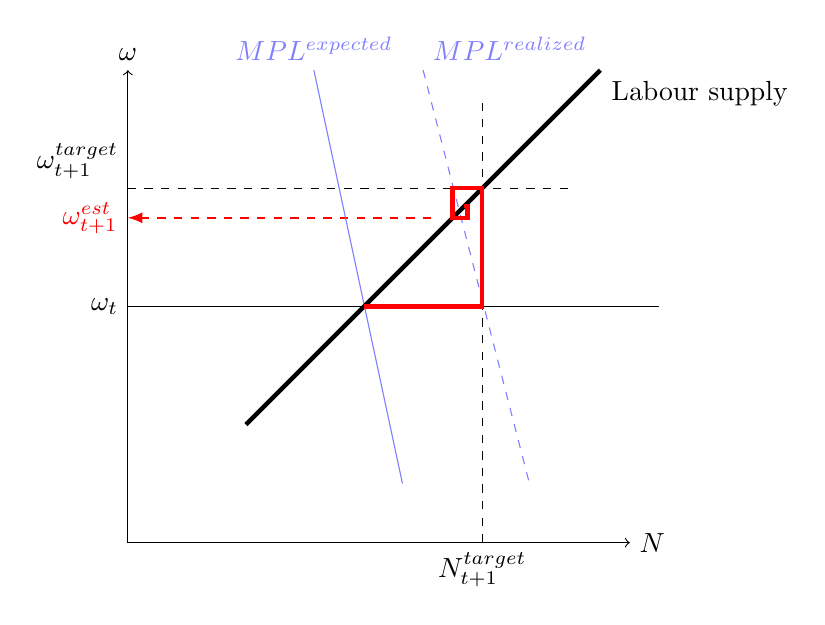
\begin{tikzpicture}[scale=.75]
% \draw[style=help lines,step=0.5cm] (-4,-4) grid (4,4)        [step=0.5cm]; %   (1,2) grid +(1,1);
% \node at (0,0){x};
 \draw[->] (-4,-4) -- (4.5,-4) node[right] {$N$};%
 \draw[] (-4,0)node[left] {$\omega_t$} -- (5,0);
\draw[dashed] (-4,2)node[above left] {$\omega_{t+1}^{target}$} -- (3.5,2);

\draw[dashed, thick, red, latex-] (-4,1.5)node[ left] {$\omega_{t+1}^{est}$} -- (1.2,1.5); %NEW
\draw[dashed] (2,-4)node[below] {$N_{t+1}^{target}$} -- (2,3.5);

 \draw[->] (-4,-4) -- (-4,4) node[above] {$\omega$};
%  \draw[->,red] (8,0.05) -- (8,3.2) -- (0.1,3.2)node[left] {$F(X^*)$};

\draw [ blue!50](-.85,4)node[above]{$MPL^{expected}$}-- (.65, -3); % 
\draw [ blue!50, dashed](1,4)node[above right]{$MPL^{realized}$} -- (2.8, -3);
\draw [ ultra thick](-2,-2) -- (4, 4)node[below right]{Labour supply}; 

\draw[ red, ultra thick](0,0) -- (2,0)  -- (2,2)--(1.5,2) -- (1.5,1.5)--(1.75, 1.5) --(1.75, 1.7)-- (1.7,1.7);%--(1.7, 1.6)--(1.7, 1.6) ;% node[right] {$X$};  CYCLING
    
 \end{tikzpicture}
    \caption {Labour market adjustment}
    \label{fig:cobweb2}
\end{figure}





% \textbf{Labour force  adjustment factor $\nu$ (pronounced nu)} This is the fraction by which desired labour exceeds actual labour
% \[\nu_t =\frac{N^{target}_{t+1}-N_{t}}{N_{t}}\]
% or 
% \[\nu_t =\frac{n^{target}_{t+1}-n_{t}}{n_{t}}\]



% \subsubsection{Wage adjustment} 

% \textbf{Wage calculation}
% Firms make one decision faced with a market wage. They choose a target workforce. This is typical in \glspl{competitive market} where firms are price-takers. 


% When \textbf{aggregate} firm labour demand exceeds N, wages rise at the city level

% To get labour supply $N^s$ in terms of  $\omega$ we combine $N=f^2 *density$ and $f=2\omega/c$. 




% Common to think of the variations in local wages as variations around a mean, in this context - perfect labour market.
% We're using this number at the aggregate level, raise the market wage to a level that attracts that many. Divide available workers among the firms, then they want to raise the wage again. It's more transparent to do it at the aggregate level than at the firm level, but we still have the rising supply curve. A more detailed agent model could implement the hiring and wage adjustment mechanisms for firms directly, but the side effect of increased complication is it also can obscure the clarity of the rent results, our focus with this work. 


% {\color{red}
\section{Relationships among parameters} \label{section-firm-initial-values}


% \subsubsection{Firm $Y_{F,i}=A_Fk_i^\alpha n_i^{\beta_F}$}
% We use the familiar Cobb-Douglas production function \cite{chiangFundamentalMethodsMathematical2002} to set relationships among variables that are consistent with basic neoclassical production theory. 
% \begin{description} \item[initial urban wage premium]



% \subsubsection{Initial wage premium for urban firms}
The theory of the firm implies certain relationships among the parameters. What we're doing here actually is simply demonstrating the typical relationships used in the theory of a firm.
% }


We know from an extensive  literature that there is an urban wage premium: urban wages are a fraction larger than  rural wages A wage premium ratio defines the initial relationship between the urban wage premium and the subsistence wage, $\omega_0 = \mathrm{wage\_premium\_ratio} * \psi$. % = p*\psi $, where $p$ is selected
 %. $p$ will vary as $\omega$ evolves. 
% \item[Initial wage premium] $\omega_0=p_0*\psi$

In this section we use subscripts rural, $R$, and urban, $U$. Outside of this section, we simplify the presentation by dropping subscripts for the urban firm, since that is the focus of the analysis, and rural properties are fixed after initial calculation. 
Parameters $\beta_F$ and $\alpha_F$ are the same for both rural firms and urban firms in this model. 
%Initial values for the urban firm's production model are set so the are reasonable, relative to the properties of the urban firm. To explore urban agglomeration effects, the rural firm parameters remain fixed, while the rural firm evolves as more people work in the city. 

\subsubsection{Initial labour force for urban firms}
To set the initial urban labour force, treat it as initially approximately the same as the rural labour force,  $n_{U,0}=n_R$. % Initially, we will try values similar to the rural firm size and allow it to adjust.  %*****%may have implica=tions later for the notation

% \item[Initial urban wage] = $\omega_0=\omega_t +\psi =(1+p_0)\psi)$
%The wage  is set as the marginal product of labour for initialization of the model. 

% \textbf{NOTE: With the initial values calculated in this section $\omega$ is consistent with $N_0$.as a result, population should not grow.}

% \begin{quotation} 

\subsubsection{Initial urban scale factor}


We calculate the urban scale factor in several steps.

\begin{description}
%\item[NEED THIS? labour cost for typical rural firm] $L_R = n_R*\psi$. % This is expressed as a money quantity: e.g., 100 workers * \$40,000/worker. We do not include other labour costs or taxes.  NEED THIS?

% \item[Initial labour cost for typical urban firm] ]  $L_U = n_R(\psi+\omega_0)$.

\item[Output for typical rural firm]  
\begin{equation}Y_R=\frac{n_R*\psi}{\beta_F}\label{eqn_Rural_output}\end{equation}
Derived from the marginal productivity condition.
% In our model, this is a constant for any initial values on the RHS. Derived from the marginal productivity condition. See item~\ref{item-paramlist-firm-level} in the orange  block. The numerical calculation is done for a firm with 100 workers and a marginal product of labour of $\psi$. %I get \$20 million for those values. 


\item[Initial output for an urban firm] 
\[Y_{U, 0} = N_0^\gamma Y^R\]  
Taking the marginal product with respect to $n$, we get a useful fact that will allow us to tie down $\gamma$
\[Y_{U,0} = \frac{n_{U,0}*(\psi+\omega_0)}{\beta_F}\]
% picturing the exponential for N
% \begin{tikzpicture}
% \begin{axis}[axis lines = left, 
% %yticklabel style={/pgf/number format/.cd,fixed,precision=3}), 
% xlabel = $N$, 
% ylabel = $N^\gamma$]
% \addplot [domain=0:2000, samples=100, color=blue]
% {x^1.13};%
% %\node at(100000, 1.013){gamma=.001};
% %\addplot [domain=1000:200000, samples=100, color=red] {x^0.00001};
% \end{axis}
% \end{tikzpicture}

\item[Capital for typical rural firm] (Derived from the marginal productivity condition.)
\[k_R=  \frac{\alpha_F Y_R }{r}\]
This is also a constant.
 
\item[Initial capital for an urban firm] (Derived from the marginal productivity condition.)
\[k_{U,0}=  \frac{\alpha_F Y_{U,0} }{r}\]


This differs from capital  for the rural firm because of the term $n^\gamma$. 

% TODO WHAT? WHERE IS GAMMA


\item[Scale factor A for typical firm] 
\[A_F= \frac{Y_R}{k_R^{\alpha_F} {n_R\psi}^{\beta_F}}\]
We will assume that this is a constant used for both rural and urban production functions. 

% CUT? (The explicit function is a bit  messy but the numeric value is easily computed because we have a rural firm labour force cost, $L_R=n_R\psi$, and have calculated $Y_F$, and  $k_F$). The prefactor.

% CHANGED: SHOULD THIS BE $\alpha_F$? n RURAL OR URBAN?

\end{description}


\section{Firm level production}  
 \textbf{This section includes numerical examples.
 }


 % We develop an argument in section~\ref{section-firm-initial-values}. Here we trace that same argument with numbers (This is incorporated above.) 
We want the marginal product of labour in the rural economy at the firm level to be at least close to \$40,000.  We can create a generic rural firm and then consider an urban firm with agglomeration effects to get the parameters we need. 

Firm employment $L$ is small relative to  urban employment {N}. Assume it is 100 workers. 

Assume that the rural production function is: 

\[ Y_{iF}^R=A_{F} K^{\alpha_F} L_F^{\beta_F}, \]

where $Y$ is the value of output, $L_F=n*\psi$, $K=r*k$.\footnote{These values give us diminishing marginal product at the firm level. If we require product exhaustion we have factor shares of  0.8 and 0.2 .The tricky point is that factor share are 
 $\frac{\alpha}{\alpha + \beta}$ and $\frac{\beta}{\alpha + \beta}$
(*If not there is surplus profit  which we will ignore.)}
Further assume that $\alpha_F=0.18 $,  and $\beta_F=0.76$. Notice that the value-MPL is the partial derivative with respect to $n$ and not L. 
The marginal products of labour and capital are: 
\[MPL=n*\beta_F Y_F/L_F=\$40,000\] and\[\ MPK=\alpha_F Y_F/K_F =0.05.\]
From the equation for the marginal product of labour, using the hypothetical initial values, we get a value of output for our rural firm:

\[Y_F=\frac{n*\psi}{\beta_F}=\frac{100*\$40,000}{0.72}=\$5,555,556.\]
This is firm revenue. From the MPK, we get the value of capital used by the firm.\footnote{The firm pays 5\% per year in capital costs,.} 

\[K_F=  \frac{\alpha_F Y_F }{r}=\frac{0.18 *\$5.5555\ million}{0.05} =\$20\ million. \]

We now have the capital, labour and output for a model firm with a marginal product of labour  equal to the subsistence wage we have chosen. We can calculate the \textbf{scale factor} $A$.

\begin{equation}  
A_F= \frac{Y_F}{K^{\alpha_F} L^{\beta_F}}=\frac{5,555,000}
{(0.05*20,000,000)^{\alpha_F} (40,000*100)^{\beta_F}} =53.34721. \label{eqn-AR}\end{equation} 

%
$A_F$ can be computed using equation~\ref{eqn-AR} for any set of coefficients and firm size.\footnote{Furthermore, we can compute the output for a city of size N if it consists of $N/n$ firms of this type. With a population of, for example 10,000. Based on the model of the rural firm above,   there would have to be  100 firms and an output of \$555,555,600$N^\gamma$. This is offered simply to see if the initial values we work with are plausible.}


\subsubsection{The urban level of production}
% \textbf{This section now redundant and has been commented out}
We now consider a firm with the same production function that operates in the city and enjoys  urban agglomeration benefits as an externality. The value of the  marginal product of labour must rise to $\psi+\omega$. We to know  the urban wage premium that is consistent with the subsistence wage.\footnote{Papageorgiou \cite{papageorgiouOccupationalMatchingCities2022} found a 4.1\% premium. D'costa and Overman show that working in London is associated with a 35.5\% higher wage than working in a rural area. The comparable figures are 10.6\% for big cities and 8.3\% for small cities and an elasticity of wages with respect to city size of 1.6\%. Estimates of the premium are lower  when controlling for individual city characteristics.}   

If the scale coefficient = 0.12 $=\omega$ would be $1.12*\psi$, or $4,800$.

We need to have a population size or a number of firms with a firm size. Assume the population is 10,000 and firms still have 100 workers. (All firms will have the same marginal product of labour in a competitive labour market, so using a representative firm should not affect our calculated values .)

\[y_C=A_F N^\gamma k^\alpha n^\beta = N^\gamma y_R\]
where $N^\gamma$ represents the agglomeration effect. This assumes that all urban production is generated by the firms and they use the same quantities of capital and labour as rural firms. Total urban production is then approximately $Fy_C=FN^\gamma y_R $, where F is the number of firms.

The marginal product of labour is 
\[MPL^u=\$44,800=N^\gamma \beta y^R/L=N^\gamma *\$40,000\]
so $N^\gamma= 1.12$ and $\gamma = \frac{log(1.12)}{log(10,000)} =  0.012$. 


To get a  $\gamma$  consistent with an empirical  value for  the wage premium  $\omega / \psi$, 
\begin{equation}
\gamma= \frac{log(1+\omega/\psi)}{log(N_0)}.\label{eqn:gamma-define}
\end{equation}


This value is consistent with an empirical  value for beta city (the urban scale exponent) of $\beta =  1.012$. The value is much lower than empirical estimates. Furthermore, if we consider the same firm structure and a population of one, the value falls, which suggests that agglomeration effects are not scale-independent, but instead increase with urban size. $\beta$ may itself be a function of $N$.\footnote{Tørsløv et al \cite{torslovMissingProfitsNations2023} show that affiliates of foreign multinational firms are an order of magnitude more profitable than local firms in a number of low-tax countries. Leveraging this differential profitability, they estimate that 36\% of multinational profits are shifted to tax havens globally. US multinationals shift twice as much profit as other multinationals relative to the size of their foreign earnings.}

% A second interesting possible implication of our calculation is that only part of the agglomeration effect appears in wages. Urban rents  are large, but agglomeration effects are much larger.
% \end{quotation}






% \textbf{appendix-05-agglomeration-model - REDUNDANT} %\renewcommand{\sfdefault}{phv}

\section{Initial values for  the agglomeration parameter}
A segment is now redundant and has been commented out

\vspace{5lines}

% {\Large  $Prefactor = 1506.712$ based on width=height=10 and density=100} and agglomeration\_coefficient= 1.2,
% We need to get the scales of the parameters and the population size roughly consistent.

% I assume the 10X10 grid is full. 

% \section{Computing the prefactor: details}
% We have set the subsistence\_wage to \$40,000.

% The urban wage premium is in the range of 13-20\%  Assume 20\% and we get \$8,000

% Under the neoclassical assumption  \$40,000 is the  marginal productivity of rural worker

% The urban production function is 
% \[Y=AN^\beta\]
% \[Y=prefactor*working\_population**scaling\_exponent\]

% where $working\_population = width*height*density$ 

% so 
% \[Y=prefactorA*(width*height*density)^{\beta}\]

% We have more conditions that this has to satisfy: The marginal product must be consistent with the urban wage and the distribution rule. The wage cannot add up to more than total output output. Workers cannot get 1.2Y/N, for example. With CRS they would get 0.8Y/N.    

% \subsection{approach one: from agglomeration surplus}
% \[urban\_wage= subsistence\_wage + wage\_share * agglomeration\_surlpus\]
% The \textbf{agglomeration surplus} is the excess relative to the CRS case when $\beta=1$:
% \[agglomeration\_surplus= A(N^{1.2} -N^1) \]
% The urban wage premium is then the share for each worker:
% \[\omega= wage\_share * \frac{agglomeration\_surlpus}{N}\]

% and this becomes
% \[\omega= wage\_share * A\left(\frac{N^{1.2}-N^1}{N}\right)=1 * A\left(N^{0.2}-1\right)\]

% To see what this looks like, consider a population of 10,000 when  wage\_share=1
% \[\omega= \$8,000 = A\left( 6.309-1 \right)\]

% {\Large So $A = 1506.712$ based on width=height=10 and density=100}  

% Smaller N makes A bigger

% % Say width=height=15 and density= 200:
% % \[\omega= \$8,000 = A\left(10000-1\right)\]

% \subsection{Approach 2: from Marginal product and subsistance wage}
% % We want the marginal product of labour in the rural economy at the firm level to be at least close to \$40,000.

% % Firm employment $L$ is small relative to  urban employment {N}.  We can create a generic rural firm and then consider an urban firm with agglomeration effects to get the parameters we need. 

% % Assume that the rural p[rooduction function is 
% % \[Y^R=A^R K^\alpha L^\beta\]
% % where $\alpha=0.2$  and $\beta=0.8$. The marginal products are 
% % \[MPL=\beta Y/L=\$40,000\] and\[\ MPK=\alpha Y/K =0.05\]
% % From the first, 

% % \[Y=\frac{L*\$40,000}{0.8}=\$5\ million\]

% % This is firm revenue. From the MPK, 

% % \[ \frac{0.2 \$5\ million}{0.05}=K =\$20\ million \]

% % We now have the capital, labour and output for a model firm with a marginal product of labour  equal to the subsistence wage we have chosen.

% % We now consider that this firm operates in the city and enjoys  urban agglomeration benefits.  If the scale coefficient=1.12$,$ $\omega$ would be as a first appr Say that the marginal product rises to \$48,000. This supports an urban wage premium of $\omega\$8,000$.

% % We need to have a population size or a number of firms with a firm size. Assume the population is 10,000 and firms have 100 workers. All firms will have the same marginal product of labour in a competitive labour market, so size should not matter. 

% % \[Y^U=A^R N^\gamma K^\alpha L^\beta = N^\gamma Y^R\]
% % with a marginal product of 
% % \[MPL^u=\$48,000=N^\gamma \beta Y^R/L=N^\gamma *\$40,000\]
% % so $N^\gamma=1.2$ and $\gamma = .019$. 


% This value is consistent with an empirical  value for $\beta$   1.02. The value is lower than empirical estimates. Furthermore, if we consider the same firm structure and a population of one million the value falls, which suggests that agglomeration effects are not scale-independent, but instead increase with urban size. $\beta$ may itself be a function of $N$.

% A second interesting possible implication of our calculation is that only part of the agglomeration effect appears in wages. Urban rents  are large, but agglomeration effects are much larger.


 

% %\[subsistance_wage= MPL(\beta=.= \]
 % bbbb{appendix-05-agglomeration model}



% \begin{enumerate}
% \item To start with a population of around 10,000, we begin with width = 10, height = 10 and density per unit of 100. 

% \item If we arbitrarily assume an initial wage premium around 20\%, and wish to start near equilibrium, % bettencourt assumed aggomeration exponent is indepent)
% we can select transportation costs. A transportation cost of 0.1  would give a distance of $\omega/.01$, which is huge. Could this be 1/10 of the starting wage premium $\omega_0$? It would then be \$800 per year, per unit distance and would give us height and width of 10. 
% % (divide into omega) - we want to start close to equilibirum. omega/cost = width
% % \item We should have a 20\% wage premium of about \$8000 to be consistent with the subsistance wage. % since we are assuming a wage premium of around 20%. Total wage has to be subsistence wage + wage premium, think of an average rural subsistence wage seems like 45K. 

% % \item Your proposed prefactor was 0.2,  251. It should be very large, based on the above numbers and the consistency constraints. I get 1507 in appendix-05-agglomeration model



% \end{enumerate}

% \subsection{Workers share}
% % The worker's of the surplus, $lambda$ It might be 0.8. It is used in...

% NOTE: 0.8 is the value of beta in a Cobb-Douglas, corresponding to the wage-share in production. It is the value used in Lobo et al


\end{document}